\documentclass[a4paper,10pt]{article}
\usepackage[T2A]{fontenc}
\usepackage[utf8x]{inputenc}
\usepackage{ucs}
\usepackage{cmap}
\usepackage[english,russian]{babel}
\usepackage{amsmath}
\usepackage{color,graphicx}
\usepackage{indentfirst}
\usepackage{ucs} 
\usepackage[utf8x]{inputenc}

\title{Обзор спайковых сетей}
\author{Чернышев Алексей}
\setlength{\parindent}{1cm}
\def\la{\left\langle\rule{0pt}{3em}}
\def\ra{\right\rangle}
\newcommand{\HRule}{\rule{\linewidth}{0.5mm}}



\begin{document}
\begin{titlepage}
\begin{center}
% Title
\HRule \\[0.4cm]
{ \huge \bfseries Cпайковые нейронные сети \\[0.4cm] }

\HRule \\[1.5cm]
% Author and supervisor
\begin{minipage}{0.4\textwidth}
\begin{flushleft} \large
\emph{Автор:}\\
асп. Чернышев Алексей
\end{flushleft}
\end{minipage}
\begin{minipage}{0.4\textwidth}
\begin{flushright} \large
\emph{Научный руководитель:} \\
д.ф.-т.н. Карпенко А.П.
\end{flushright}
\end{minipage}

\vfill

% Bottom of the page
{\large Август 2014}

\end{center}
\end{titlepage}


\tableofcontents
\clearpage
\section{Введение}

\section{Биологическая основа нейронов}
\indent Человеческий мозг содержит в себе огромное количество соединенных между собой нейронов, нервных клеток, которые стали предметом интереса во многих областях, таких как нейрофизиология, теоретическая нейронаука, искусственный интеллект.\\
\indent Нейрон по своему строению довольно схож с другими клетками: тело нейрона окружено плазматической мембраной, внутри которой находятся ядро, цитоплазма и другие составляющие клетки. Однако, нейрон несет в себе особую функцию: нейрон выполняет приём сигналов от других нейронов, выполняет их преобразование и передает их на вход другим нейронам или клеткам. Сигнал представляет из себя импульсы нервной активности, имеющих электрохимическую природу\\
\indent Нейроны крайне разнообразные по форме и нюансам функционирования, хотя существует возможность вывести наиболее типичную форму нейрона. На рис. \ref{bio_pic} отображена схема биологического нейрона. \\
\begin{figure}[ht]
\centering
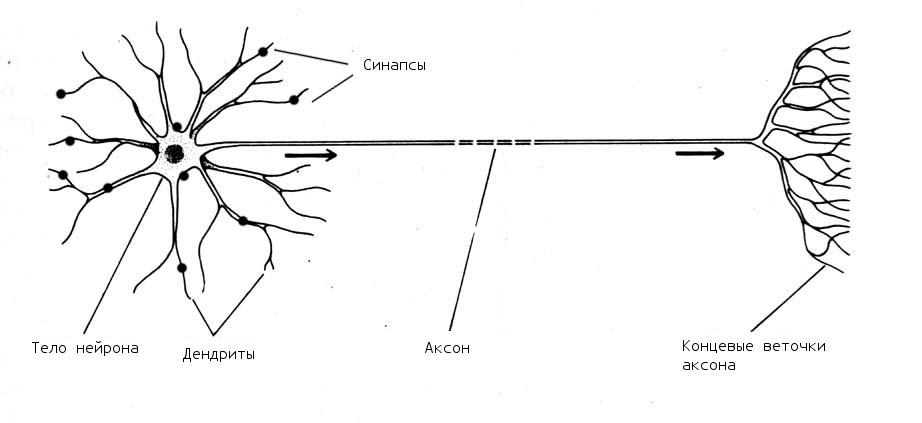
\includegraphics[width=1\linewidth]{bio_neuron.jpg}
\caption{биологический нейрон}
\label{bio_pic}
\end{figure} \\
\indent Прием нервных импульсов от других нейронов происходит посредством дендритов, на которых расположены синапсы - точки соединения нейронов между собой. Дендриты проводят входные импульсы с синапсов доставляя их клетке нейрона, которые специфичным образом возбуждают клеточную мембрану.\\
\indent Элетрохимические процессы внутри клетки делают нейрон в той или иной мере чувствительным к возбужденям мембраны, и когда возбуждение достигает определенного порога, потенциал на мембране на короткое время (около 2 мс) осуществляет резкий скачок вверх, порождая короткий импульс называемый спайком. После выработки спайка нейрон переживает т.н. рефракторный период, в течении которого чувствительность мембраны к возбуждениям резко спадает.\\
\indent Синапсы, при более подробном взгляде, представляют из себя не менее сложный механизм, чем сама клетка нейрона. Типичный синапс, как контакт между двумя нейронами, представляет собой пузырек наполненный нейромедиаторами находящийся на аксоне пресинапатической клетки и мембрана чувствительная к нейромедиаторам на дендрите постсинаптической клетки. При возмбуждении аксона нейромедиаторы синапса начинают освобождаться в пространство между пресинаптической и постсинаптической мембраной - синаптическую щель (10-50 нм), где они встречаются с чувствительными белками на постсинаптической мембране. Следствием такой структуры является односторонее проведение нервного импульса. Количество высвобожденного и принятого нейромедиатора варьируется, и ``натренированный'' синапс, будет проводить гораздо большее количество импульса засчёт большего количество нейромедиаторов в синаптическом пузырьке и на постсинаптической мембране. В нейроинформатике, обычно, пренебрегают такими тонкими деталями, и вводят ``веc'' синапса, который характеризует насколько эффективно синапс может проводить импульс.\\
\indent Ещё один феномен касающийся нюансов функционирования биологического нейрона - сенсорная адаптация\cite{Phizi}. Нейрон при получении импульсов с одной и той же характеристикой, как правило, начинает ``привыкать'' и начинает  приспосабливаться, чтобы тратить меньше энергии при интеграции этого сигнала. Как следствие, интенсивность его ответа угасает. Исследователями в области теоретической нейронауки этот феномен довольно пристально исследуется и существуют выводы об оптимальности такого поведения, с точки зрения оптимизации переданной информации нейроном \cite{Adapt,TripleAdapt}.

\subsection{Модель Ходжкина-Хаксли}
	В 1952 году Алан Ллойд Ходжкин и Эндрю Хаксли разработали первую, наиболее подробную на тот момент математическую модель нейрона. Модель была построена на основе динамики генерации и передачи нервного сигнала в гигантcком аксоне кальмара.\\
	\indent Данную модель сложно применить в решении реальных задач, которые решает нейроинформатика, так как её моделирование ресурсоёмко - около 1200 операций с плавающей точкой для моделирования одной милисекунды\cite{BohteReview}. Однако, модель играет важную научную и историческую роль в нейронауках.\\
	\indent Общая динамика потенциала нейрона описывается плавным затуханием значения потенциала на мембране $u_{m}(t)$, со скоростью, которая характеризуется ёмкостью мембраны $C_{m}$
	\begin{equation}\label{eq:hh}
	C_{m}\frac{du_{m}(t)}{dt}+I_{ion}(t)=I_{ext}(t).
	\end{equation}	 
	\indent Здесь $I_{ion}(t)$ - сумма ионных токов внутри клетки, $I_{ext}(t)$ - приложенный ток снаружи клетки.\\
	\indent Сложность уравнения \eqref{eq:hh_ion}	 таится в моделировании ионных токов для каждого типа ионов. В модели Ходжкина-Хаксли динамика ионных токов характеризуется наличием т.н. ионных каналов, открытие или закрытие которых влияет на общую динамику напряжения на мембране. В исходной модели Ходжкина-Хаксли было два вида ионов $Na^{+}$ и $K^{-}$, где ионный поток $Na^{+}$ описывается тремя каналами вероятность открытия которых $p_{m}$ и одним каналом с вероятностью открытия $p_{h}$, ионный поток $K^{-}$ описывается четырьмя каналами с вероятностью открытия $p_{n}$\cite{Genesis}.\\ 
	\indent Динамика вероятности открытия-закрытия каналов, выражается дифференциальным уравнением первого порядка
	\begin{equation}\label{eq:hh_pch}
	\frac{dp_{i}(t)}{dt} = \alpha_{i}(u_{m}(t))(1-p_{i}(t)) - \beta_{i}(u_{m}(t))p_{i}(t),
	\end{equation}	 
	где $\alpha_{i}(u_{m}(t)), \beta_{i}(u_{m}(t))$ константы зависящие от потенциала на мембране, которые характеризуют скорость закрытия и открытия канала, соответственно. Временной промежуток, спустя который вероятность достигает равновесия, описывается константой
	\begin{equation}\label{eq:hh_t}
	\tau_{i}=\frac{1}{\alpha_{i}(u_{m}(t))+\beta_{i}(u_{m}(t))}	
	\end{equation}
	\indent Таким образом динамику ионных токов для модели Ходжкина-Хаксли, можно описать уравнением
	\begin{align}\label{eq:hh_ion}
	I_{ion}(t) &= \begin{aligned}[t]
	&\bar{g}_{Na}\;p_{m}^{\;3}(t)\;p_{h}(t)\;(u_{m}(t)-E_{Na}) +	\\
	+\;&\bar{g}_{K}\;p_{n}^{\;4}(t)\;(u_{m}(t)-E_{K})+\bar{g}_{L}(u_{m}(t)-E_{L})	\\
	\end{aligned}
	\end{align}
	где $p_{m}(t), p_{h}(t), p_{n}(t)$ - вероятности открытия каналов, описываются уравнением динамики \eqref{eq:hh_pch}, которые включают соответствующие константы. Смысл и значения констант можно найти в оригинальной работе\cite{HH}.\\
	\indent Не смотря на то что применение такой модели в задачах машинного обучения затруднительно, ввиду её сложности, эта модель играет свою важную как научную, так и историческую роль.

\section{Модели нейронов}
\subsection{Нейронные сети в нейроинформатике}
\subsubsection{Нейрон МакКалока-Питтса}
   Первая модель нейрона, положившая начало нейроинформатике  - модель МакКаллока-Питтса. Эта модель прочно заложила фундамент теории нейронных сетей, и исследования новых свойств этой модели не   прекращаются по сей день.\\
   \indent Впервые, была реализована идея использовать нейрон, как вычислительный элемент. Раннее развитие данного направления в основном характеризуется попыткой рассмотреть нейроны, как элементы,        реализующие простейшие логические операции или преобразования. Впоследствии были созданы более сложные схемы, в которых данный нейрон соединяется в сети.\\
   \indent Ключевой особенностью данной модели является то, что нейрон представляется, как взвешенный сумматор входных скалярных признаков $\boldsymbol{x}=(x_{1},x_{2},...,x_{n})$. Обработка нейроном входов происходит пропусканием взвешенной суммы через нелинейную функцию $\phi(x)$, называемую функцией активации\\
   \begin{equation}\label{eq:sum_mp}
   \boldsymbol{y}(x) = \phi(\sum_{j=1}^{n}w_{j}x_{j}).
   \end{equation}
\indent Здесь $\boldsymbol{w}=(w_{1}, w_{2},...,w_{n})$ выражает вектор весов взвешенного сумматора (синапсов нейрона), $y(x)$ - выходной результат обработки нейроном вектора $\boldsymbol{x}$.\\	
	\indent В качестве нейлинейной функции, наиболее популярным выбором является сигмоидальная функция\cite{Zaencev1999}. Данная функция удобна своей непрерывностью и гладкостью, и позволяет ограничить выход нейрона  отрезком значений $y(x)\in[0,1]$, такой выход можно интерпретировать как уровень активации нейрона, в зависимости от входного вектора $\boldsymbol{x}$ и настройки весов $\boldsymbol{w}$, что имеет свою, пускай и отдаленную, биологическую подоплёку. \\
   \indent Не смотря на ошеломляющий успех и широкое применения данной модели  и производных моделей в прикладных задачах, с биологической точки зрения такие нейроны, только отдаленно напоминают, то как работают настоящие нейроны в мозгу.\\
   \indent Важным отличием такого нейрона от биологического является тот факт, что данная модель не имеет внутреннего состояния и не может быть представлена в виде динамической системы\cite{Zaencev1999}. Данное свойство серьезно ограничивает круг задач в которых можно было бы применить нейронные сети. 

\subsection{Формальные спайковые модели}   
\indent Нейронные модели описанные в данной секции принадлежат к семейству формальных моделей. Простота этих моделей позволяет перейти от анализа одного-двух нейронов к анализу популяций нейронов соединённых в сети, опуская биологическую точность, но сохраняя общие черты характерные для биологических нейронов.\\
\subsubsection{Модель Integrate-and-Fire}

\indent Модель Integrate-and-fire имеет большую историю. Ещё в 1907 году 	французский физиолог Луи Лапик эксперементируя с лягушками описал модель возбуждения нервных клеток используя RC-цепь\cite{Lapicque}. За свою вековую историю модель, благодаря своей простоте и, главное, биологической оправданности, получила много применений.\\
   \indent Динамика модели описывается динамической системой с одной переменной, довольно похожей на уравнение \eqref{eq:hh}, за тем исключением, что ионные токи не моделируются, а спайк генерируется нейроном при достижении заранее заданного порога:\\
   \begin{equation}\label{eq:iaf}
   \begin{split}
   \tau_{m}\frac{du}{dt}&=-u(t)+R I(t),\\
   t^{(f)}: u(t^{(f)}) &= \vartheta 
   \end{split}
   \end{equation}
где $t^{f}$ - время спайка, $\vartheta$ - порог напряжения, временная константа мембраны $\tau_{m}=RC$, $R$ и $C$ - сопротивление и ёмкость RC-цепи соответственно, $I(t)$ - приложенный ток извне.\\   
\indent Данная нейронная модель подходит для конструирования нейронных сетей: приложенный ток $I(t)$ можно рассмотреть, как ток, получаемый нейроном через синапсы от других нейронов. Допустим нейрон соединён с N входными спайковыми нейронами синапсами с определенными весами, тогда приложенный ток можно описать:
\begin{equation}\label{eq:iaf_syn}
I(t) = \sum_{j=1}^{N} w_{j}\; \epsilon(t-t_{j}^{f})
\end{equation}
где $\epsilon(t)$ - низкочастотный фильтр, как правило, в виде затухающей экспоненты, который характеризует спайк на синапсе, такая функция хорошо описывает импульс переданный в процессе передачи нейромедиаторов, $w_{j}$ - скаляр выражающий вес на синапсе, $t_{j}^{f}$ - спайк не входном нейроне.\\

\subsubsection{Модель Ижикевича}
Модель нейрона в виде динамической системы с двумя переменными, довольно проста и в то же время имеет богатую динамику. Модель является компромиссом между упрощенной моделью IaF и HH. 

\subsubsection{Spike Response Model}
Отдельным рядом стоит модель SRM, в своём оригинальном виде модель повторяет IaF, но в своей формулировке наиболее удобна для теоретического исследования. Наиболее часто эту модель используют со   стохастическим порогом, который позволяет процесс генерации спайка описать негомогенным пуассоновским процессом.

\subsubsection{Spike Response Model с адаптацией}
Усложнение модели SRM, которая повторяет феномен адаптации.

\section{Обучение с учителем и без учителя}
\subsection{Классическое правило Хэбба}
\subsection{Обучение на основе градиента ошибки}
\subsection{Обучение на основе феноменологической модели STDP}
\subsection{Теоретическая оптимальная модель STDP}
\section{Обучение с подкреплением}
\subsection{Трехфакторное правило обучения}
\subsection{Гедонистический синапс}
\subsection{Обучение на основе TD-ошибки}
\section{Выводы}
\section{Использованная литература}
\bibliography{refs}{}
\bibliographystyle{unsrt}

\end{document}
